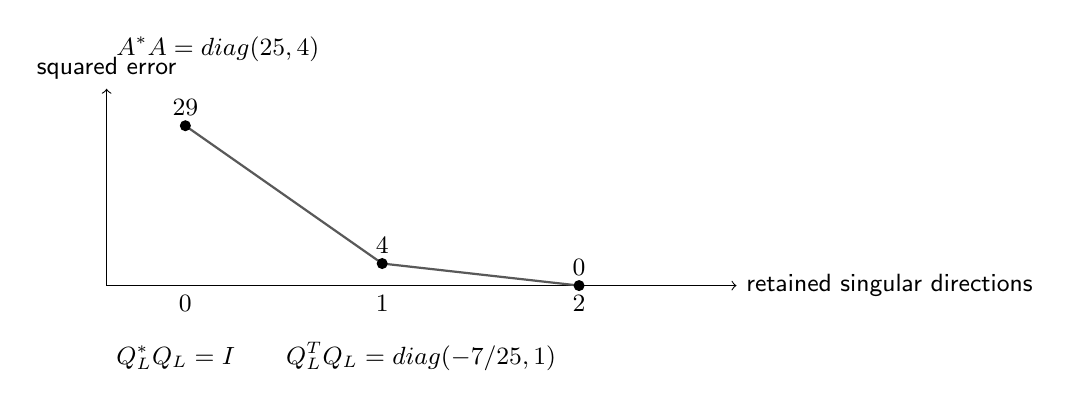
\begin{tikzpicture}[font=\sffamily\small]
\node[anchor=west] at (0,3) {$A^*A=\operatorname{diag}(25,4)$};
\draw[->] (0,0)--(8,0) node[right] {retained singular directions};
\draw[->] (0,0)--(0,2.5) node[above] {squared error};
\draw[thick,black!65] (1,2.03)--(3.5,.28)--(6,0);
\foreach \x/\y/\n/\v in {1/2.03/0/29,3.5/.28/1/4,6/0/2/0}{
\fill (\x,\y) circle (2pt);\node[below] at (\x,0) {$\n$};\node[above] at (\x,\y) {$\v$};}
\node[anchor=west] at (0,-.9) {$Q_L^*Q_L=I\qquad Q_L^TQ_L=\operatorname{diag}(-7/25,1)$};
\end{tikzpicture}
